\documentclass[a4paper, 12pt]{article}
\usepackage[T1]{fontenc}
\usepackage[utf8]{inputenc}
\usepackage[italian]{babel}

%Risolve il problema di Adobe Reader che vedevo i caratteri dell'indice un po' grigi, non riuscendo a leggerli bene
\usepackage{lmodern}

\usepackage{natbib}
\usepackage{graphicx}

\usepackage{color}
\definecolor{myGreen}{rgb}{0,0.69,0.313}
\definecolor{myBlue}{rgb}{0.2157,0.3765,0.5725}
\definecolor{myBrown}{rgb}{0.59215,0.28235,0.02353}

\usepackage{listings}
\lstdefinelanguage{SQL}
{keywords={CREATE, SCHEMA, TABLE, AUTHORIZATION, REFERENCES, UNIQUE, PRIMARY, KEY, FOREIGN, DOMAIN, DELETE, ON, UPDATE, DEFAULT, CONSTRAINT, NOT, NULL, CHECK, AND, OR, CASCADE, SELECT, FROM, WHERE},
	keywordstyle={\bfseries},
	columns=fixed,
	sensitive=false,
	showtabs=false,
	showspaces=false,
	tabsize=4,
	captionpos=b,
	basicstyle={\sffamily}
}
%Tabelle
\usepackage{tabularx}
\usepackage{booktabs}
\usepackage{tabu}
\usepackage{caption} 
\captionsetup[table]{skip=2pt}
\setlength\arrayrulewidth{1pt}


%Serve per avere l'indice cliccabile. Con questi parametri inoltre non spuntano i riquadri rossi di default
%TODO Non dimenticare di togliere il commento su hyperref quando finisco la relazione
%\usepackage[colorlinks=true, linkcolor=black, citecolor=black, urlcolor=black]{hyperref}

% Impostazioni di pagina e margini
\usepackage[a4paper, margin=2.54cm]{geometry}

%Header and Footer
\usepackage{fancyhdr}
\pagestyle{fancy}
\fancyhf{}
\lhead{TIW - Gestione Preventivi - a.a. 2021/2022}
\cfoot{\thepage}
%warning per 12pt del carattere
\setlength{\headheight}{14.49998pt}
\addtolength{\topmargin}{-2.49998pt}
% Titolo e informazioni
\title{TIW - Gestione Preventivi}
\author{Riccardo Inghilleri - Matricola n. 937011\\Manuela Merlo - Matricola n. 936925}
\date{Anno Accademico 2021/2022}

\begin{document}
\begin{titlepage}
	\begin{center}
		\vspace*{1cm}
		
		\Huge
		TIW - Gestione preventivi pure HTML\\
		\vspace{4cm}
		
		
\includegraphics[width=0.4\textwidth]{polimilogo}
		
		\vspace{3.5cm}
		\LARGE
		Politecnico di Milano\\
		Anno Accademico 2021/2022\\
		\vspace{0.5cm}
		\Large
		Prof. Piero Fraternali\\
		
		\vspace{5cm}
		
		{Riccardo Inghilleri (Codice Persona 10713236 - Matricola 937011)\\Manuela Merlo (Codice Persona 10670533 - Matricola 936925)}
		
		\vfill
		
		\vspace{0.8cm}
		
	\end{center}
\end{titlepage}
\tableofcontents
\newpage
\section{Gestione Preventivi - Pure HTML}
\subsection{Analisi dei dati per il database} \label{sub: Analisi dei dati per il database}
Un’applicazione web consente la gestione di richieste di preventivi per prodotti personalizzati. L’applicazione supporta registrazione e login di \textbf{\textcolor{red}{clienti}} e \textbf{\textcolor{red}{impiegati}} mediante una pagina pubblica con opportune form. La registrazione controlla l’unicità dello \textbf{\textcolor{myGreen}{username}}. Un \textbf{\textcolor{red}{preventivo}} \textbf{\textcolor{myBlue}{è associato a un}} \textbf{\textcolor{red}{prodotto}}, \textbf{\textcolor{myBlue}{al cliente che l’ha richiesto}} e \textbf{\textcolor{myBlue}{all’impiegato che l’ha gestito}}. Il preventivo \textbf{\textcolor{myBlue}{comprende una o più} \textcolor{red}{opzioni} \textcolor{myBlue}{per il prodotto a cui è associato}}, che devono essere tra quelle disponibili per il prodotto. Un prodotto ha un \textbf{\textcolor{myGreen}{codice}}, un’\textbf{\textcolor{myGreen}{immagine}} e un \textbf{\textcolor{myGreen}{nome}}. Un’opzione ha un \textbf{\textcolor{myGreen}{codice}}, un \textbf{\textcolor{myGreen}{tipo}} (“normale”, “in offerta”) e un \textbf{\textcolor{myGreen}{nome}}. Un preventivo ha un \textbf{\textcolor{myGreen}{prezzo}}, definito dall’impiegato. Quando l’utente (cliente o impiegato) accede all’applicazione, appare una LOGIN PAGE, mediante la quale l’utente si autentica con username e \textbf{\textcolor{myGreen}{password}}. Quando un cliente fa login, accede a una pagina HOME PAGE CLIENTE che contiene una form per creare un preventivo e l’elenco dei preventivi creati dal cliente. Selezionando uno dei preventivi il cliente ne visualizza i dettagli. Mediante la form di creazione di un preventivo l’utente per prima cosa sceglie il prodotto; scelto il prodotto, la form mostra le opzioni di quel prodotto. L’utente sceglie le opzioni (almeno una) e conferma l’invio del preventivo mediante il bottone INVIA PREVENTIVO. Quando un impiegato effettua il login, accede a una pagina HOME PAGE IMPIEGATO che contiene l’elenco dei preventivi gestiti da lui in precedenza e quello dei preventivi non ancora associati a nessun impiegato. Quando l’impiegato seleziona un elemento dall’elenco dei preventivi non ancora associati a nessuno, compare una pagina PREZZA PREVENTIVO che mostra i dati del cliente (username) e del preventivo e una form per inserire il prezzo del preventivo. Quando l’impiegato inserisce il prezzo e invia i dati con il bottone INVIA PREZZO, compare di nuovo la pagina HOME PAGE IMPIEGATO con gli elenchi dei preventivi aggiornati. Il prezzo definito dall’impiegato risulta visibile al cliente quando questi accede all’elenco dei propri preventivi e visualizza i dettagli del preventivo. La pagina PREZZA PREVENTIVO contiene anche un collegamento per tornare alla HOME PAGE IMPIEGATO. L’applicazione consente il logout dell’utente.\\

\noindent \textbf{\textcolor{red}{Entities}, \textcolor{myGreen}{attributes}, \textcolor{myBlue}{relationships}}
\newpage
\subsection{Database Design}
\begin{figure}[h!]
	\centering
	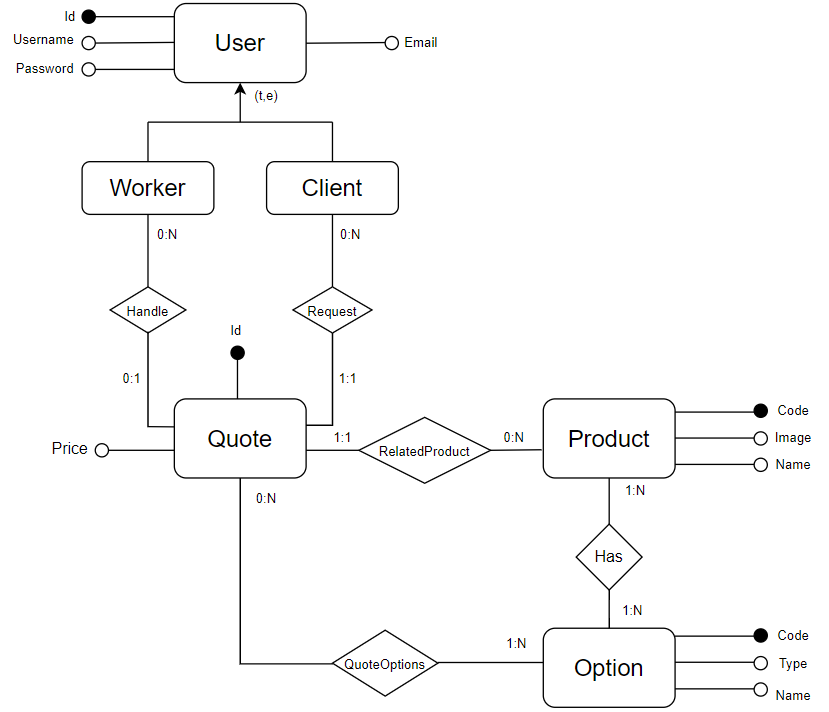
\includegraphics[width=1\textwidth]{PureHTML_images/quotemanagementdesign.png}
	\caption{Database Desing}
	\label{figure:database_design}
\end{figure}
\subsection{Local Database schema}
\begin{lstlisting}[language=SQL]
CREATE TABLE `user` (
`id` int AUTO_INCREMENT,
`username` varchar(45),
`email` varchar(255),
`password` varchar(45) NOT NULL,
`role` varchar(45) NOT NULL,
PRIMARY KEY (`id`),
UNIQUE(`email`),
CONSTRAINT `UC_UsernameRole` UNIQUE (`username`,`role`),
CONSTRAINT `NN_UsernameORRole` 
CHECK (`username` is not null OR `email` is not null))

CREATE TABLE `product` (
`code` int AUTO_INCREMENT,
`image` varchar(45) NOT NULL,
`name` varchar(45) NOT NULL,
PRIMARY KEY (`code`))


CREATE TABLE `option` (
`code` int AUTO_INCREMENT,
`type` varchar(45) NOT NULL,
`name` varchar(45) NOT NULL,
PRIMARY KEY (`code`))


CREATE TABLE `quote` (
`id` int auto_increment,
`clientId` int NOT NULL,
`workerId` int,
`productCode` int NOT NULL,
`price` int default null,
PRIMARY KEY (`id`),
CONSTRAINT `asstoclient` FOREIGN KEY (`clientId`) 
REFERENCES `client` (`id`) ON DELETE CASCADE,
CONSTRAINT `asstoworker` FOREIGN KEY (`workerId`) 
REFERENCES `worker` (`id`) ON DELETE CASCADE,
CONSTRAINT `asstoproduct` FOREIGN KEY (`productCode`) 
REFERENCES `product` (`code`) ON DELETE CASCADE)


CREATE TABLE `productoptions`(
`productCode` int,
`optionCode` int,
PRIMARY KEY (`productCode`,`optionCode`),
CONSTRAINT `relwithproduct` FOREIGN KEY (`productCode`) 
REFERENCES `product` (`code`) ON DELETE CASCADE,
CONSTRAINT `relwithoption` FOREIGN KEY (`optionCode`) 
REFERENCES `option` (`code`) ON DELETE CASCADE)


CREATE TABLE `quoteoptions`(
`quoteId` int NOT NULL,
`optionCode` int NOT NULL,
PRIMARY KEY (`quoteId`,`optionCode`),
CONSTRAINT `relwithquote` FOREIGN KEY (`quoteId`) 
REFERENCES `quote` (`id`) ON DELETE CASCADE,
CONSTRAINT `selectedoption` FOREIGN KEY (`optionCode`) 
REFERENCES `option` (`code`) ON DELETE CASCADE)
\end{lstlisting}
\subsection{Analisi dei dati per i requisiti dell'applicazione} \label{sub: Analisi dei dati per i requisiti dell'applicazione}
Un’applicazione web consente la gestione di richieste di preventivi per prodotti personalizzati. L’applicazione supporta \textbf{\textcolor{myBrown}{registrazione}} e \textbf{\textcolor{myBrown}{login}} di clienti e impiegati mediante una pagina pubblica con opportune \textbf{\textcolor{myGreen}{form}}. La registrazione controlla l’unicità dello username. Un preventivo è associato a un prodotto, al cliente che l’ha richiesto e all’impiegato che l’ha gestito. Il preventivo comprende una o più opzioni per il prodotto a cui è associato, che devono essere tra quelle disponibili per il prodotto. Un prodotto ha un codice, un’immagine e un nome. Un’opzione ha un codice, un tipo (“normale”, “in offerta”) e un nome. Un preventivo ha un prezzo, definito dall’impiegato. Quando l’utente (cliente o impiegato) \textbf{\textcolor{myBlue}{accede all’applicazione}}, \textbf{\textcolor{myBrown}{appare}} una \textbf{\textcolor{red}{LOGIN PAGE}}, mediante la quale \textbf{\textcolor{myBlue}{l’utente si autentica}} con username e password. Quando un cliente fa login, accede a una pagina \textbf{\textcolor{red}{HOME PAGE CLIENTE}} che contiene una \textbf{\textcolor{myGreen}{form}} \textbf{\textcolor{myBrown}{per creare un preventivo}} e \textbf{\textcolor{myGreen}{l’elenco dei preventivi}} creati dal cliente. \textbf{\textcolor{myBlue}{Selezionando uno dei preventivi}} il cliente ne \textbf{\textcolor{myGreen}{visualizza i dettagli}}. Mediante la form di creazione di un preventivo l’utente per prima cosa sceglie il prodotto; \textbf{\textcolor{myBlue}{scelto il prodotto}}, la form mostra \textbf{\textcolor{myGreen}{le opzioni di quel prodotto}}. L’utente sceglie le opzioni (almeno una) e \textbf{\textcolor{myBlue}{conferma l’invio}} del preventivo mediante il \textbf{\textcolor{myGreen}{bottone INVIA PREVENTIVO}}. Quando un impiegato effettua il login, accede a una pagina \textbf{\textcolor{red}{HOME PAGE IMPIEGATO}} che contiene l’\textbf{\textcolor{myGreen}{elenco dei preventivi}} gestiti da lui in precedenza e \textbf{\textcolor{myGreen}{quello dei preventivi non ancora associati}} a nessun impiegato. Quando l’impiegato \textbf{\textcolor{myBlue}{seleziona un elemento}} dall’elenco dei preventivi non ancora associati a nessuno, compare una \textbf{\textcolor{red}{pagina PREZZA PREVENTIVO}} che mostra \textbf{\textcolor{myGreen}{i dati del cliente (username) e del preventivo}} e una \textbf{\textcolor{myGreen}{form}} \textbf{\textcolor{myBrown}{per inserire il prezzo del preventivo}}. Quando l’impiegato \textbf{\textcolor{myBlue}{inserisce il prezzo e invia i dati}} con il \textbf{\textcolor{myGreen}{bottone INVIA PREZZO}}, compare di nuovo la pagina HOME PAGE IMPIEGATO con gli elenchi dei preventivi aggiornati. Il prezzo definito dall’impiegato risulta visibile al cliente quando questi \textbf{\textcolor{myBlue}{accede all’elenco dei propri preventivi}} e visualizza i dettagli del preventivo. La pagina PREZZA PREVENTIVO contiene anche un collegamento per tornare alla HOME PAGE IMPIEGATO. L’applicazione consente il \textbf{\textcolor{myBrown}{logout}} dell’utente.\\

\noindent \textbf{\textcolor{red}{Pages(views)}, \textcolor{myGreen}{views components}, \textcolor{myBlue}{events}, \textcolor{myBrown}{actions}}
\subsection{Completamento delle specifiche}
\begin{itemize}
	\item La pagina di default contiene la form di login;
	\item Lo username e la password non possono essere nulli;
	\item Un client e un worker possono avere lo stesso username, due client o due worker invece no;
	\item Il prezzo non può essere negativo;
	\item \'E permesso al client di richiedere preventivi dello stesso prodotto con le stesse opzioni;
	\item Nel caso di riapertura del sito da parte di un utente che precedentemente non ha effettuato il logout, non viene richiesta una nuova autenticazione e viene aperta direttamente la sua home page.
	\item Quando un client vuole vedere i dettagli di un preventivo, viene reindirizzato a un'altra pagina.
 
\end{itemize}
\newpage
\subsection{Application Desing}
\begin{figure}[h!]
	\centering
	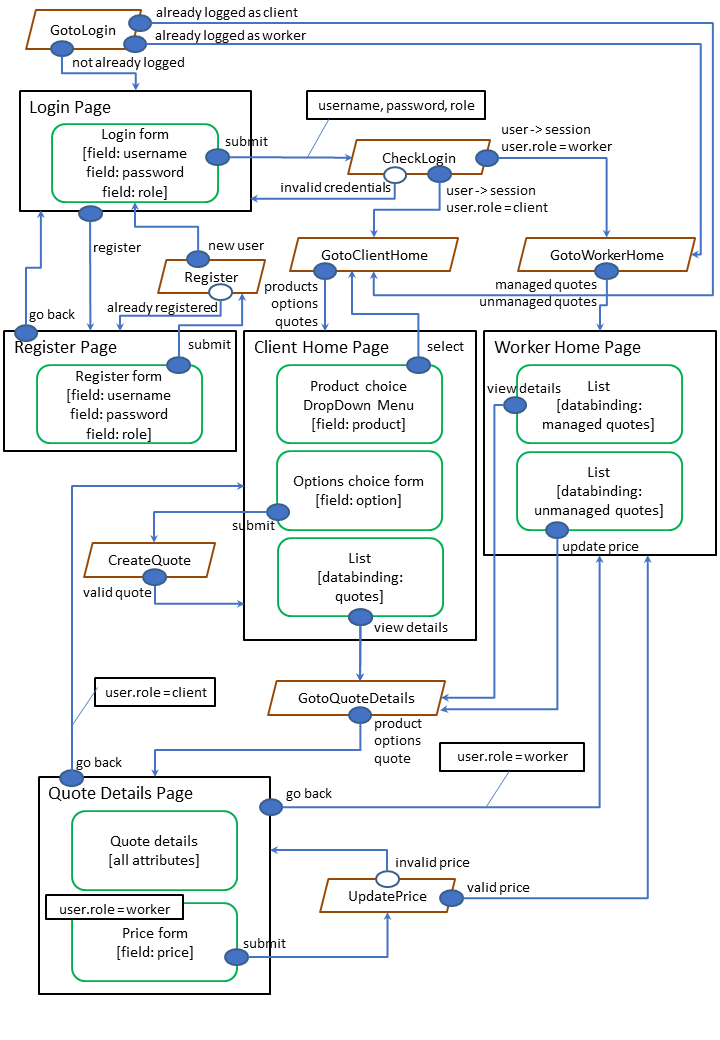
\includegraphics[width=0.97\textwidth]{PureHTML_images/ifml.png}
	\caption{IFML diagram}
	\label{figure:ifml}
\end{figure}
\newpage
\subsection{Components}

\begin{itemize}
\item \textbf{Model Objects (Beans)}
\begin{itemize}
\item Option
\item Product
\item Quote
\item User
\end{itemize}
\item \textbf{Data Access Objects (Classes)}
\begin{itemize}
	\item \textbf{OptionDAO}
	\begin{itemize}
		\item boolean hasOptionByCode(int productCode, int optionCode);
		\item List<Option> findOptionsByProductCode(int productCode);
		\item List<Option> findOptionsByQuoteId(int quoteId);
		\item void insertOption(int quoteId, int optionCode);
	\end{itemize}
	\item \textbf{ProductDAO}
	\begin{itemize}
		\item List<Product> findAllProducts();
		\item Product findProductByCode(int code);
	\end{itemize}
	\item \textbf{QuoteDAO}
	\begin{itemize}
		\item List<Quote> findQuotesByUserId(int userId, String role);
		\item Quote findQuoteById(int quoteId);
		\item List<Quote> findUnmanagedQuotes();
		\item int insertQuote(int clientId, int productCode);
		\item void updateQuote(int quoteId, int workerId, int price);
	\end{itemize}
	\item \textbf{UserDAO}
	\begin{itemize}
		\item User findUser(String username, String password, String role);
		\item User findUser(String username, String role);
		\item User findClientById(int clientId);
		\item void registerUser(String username, String password, String role);
	\end{itemize}
\end{itemize}
\item \textbf{Controllers (Servlets)}
\begin{itemize}
	\item GotoLogin
	\item CheckLogin
	\item Register
	\item GotoClientHome
	\item GotoWorkerHome
	\item CreateQuote
	\item GotoQuoteDetails
	\item UpdatePrice
	\item Logout
\end{itemize}
\item \textbf{Filters}
\begin{itemize}
	\item SessionChecker
	\item ClientChecker
	\item WorkerChecker
\end{itemize}
\item \textbf{Views (Templates)}
\begin{itemize}
\item Login.html
\item Register.html
\item ClientHome.html
\item WorkerHome.html
\item QuoteDetails.html
\end{itemize}
\end{itemize}

\subsection{Events}
I filtri utilizzati sono i seguenti:\\

\noindent \textbf{SessionChecker:}
\begin{itemize}
\item \textbf{Controllo:} session.isNew() || session.getAttribute("currentUser") == null 
\item \textbf{Azione:} redirect alla Login Page
\item \textbf{Quando:} prima di ogni Servlet
\end{itemize}
\textbf{ClientChecker:} controlla che lo user corrente sia un Client
\begin{itemize}
\item \textbf{Controllo:} !user.getRole().equals("client")
\item \textbf{Azione:} redirect alla Login Page
\item \textbf{Quando:} prima di /GotoClientHome e /CreateQuote
\end{itemize}
\textbf{WorkerChecker:} controlla che lo user corrente sia un Worker
\begin{itemize}
\item \textbf{Controllo:} !user.getRole().equals("worker")
\item \textbf{Azione:} redirect alla Login Page
\item \textbf{Quando:} prima di /GotoWorkerHome e /UpdatePrice
\end{itemize}
\newpage
\subsubsection{Go to Login}
\begin{figure}[h!]
	\centering
	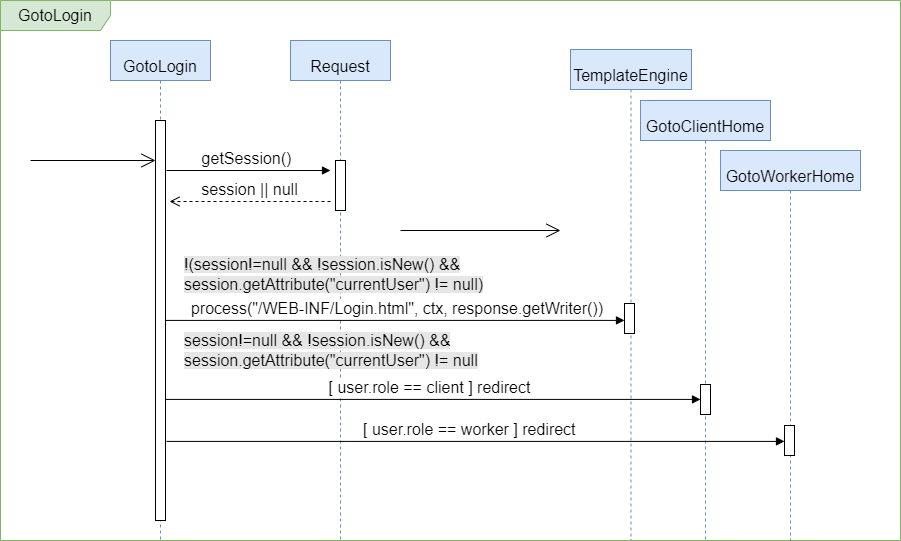
\includegraphics[width=1\textwidth]{PureHTML_images/GotoLogin.png}
	\caption{Event - Go to Login}
	\label{figure:gotologin_sd}
\end{figure}
\subsubsection{Login}
\begin{figure}[h!]
	\centering
	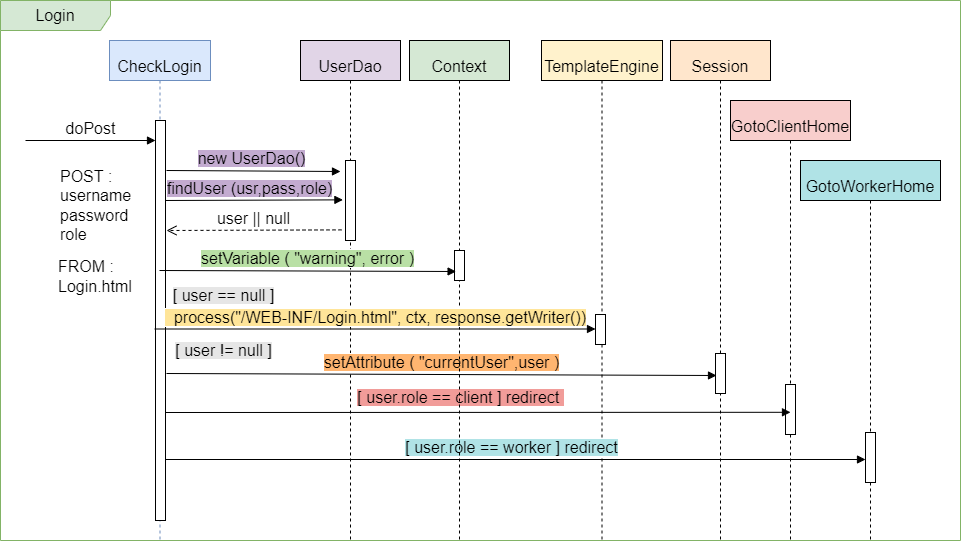
\includegraphics[width=1\textwidth]{PureHTML_images/Login.png}
	\caption{Event - Login}
	\label{figure:login_sd}
\end{figure}
\noindent \textbf{Controlli:}

\noindent \textbf{HTML:} \\ Lo username e la password sono obbligatori.

\noindent \textbf{Server:} 

\noindent Viene controllato che i parametri della Form non sia nulli, vuoti o invalidi:

\begin{lstlisting}[language=java] 
(username = null || role = null || 
(!role.equalsIgnoreCase("client") && !role.equalsIgnoreCase("worker")) 
|| password = null || 
username.isEmpty() || password.isEmpty())
\end{lstlisting}

\subsubsection{Register}
\begin{figure}[h!]
	\centering
	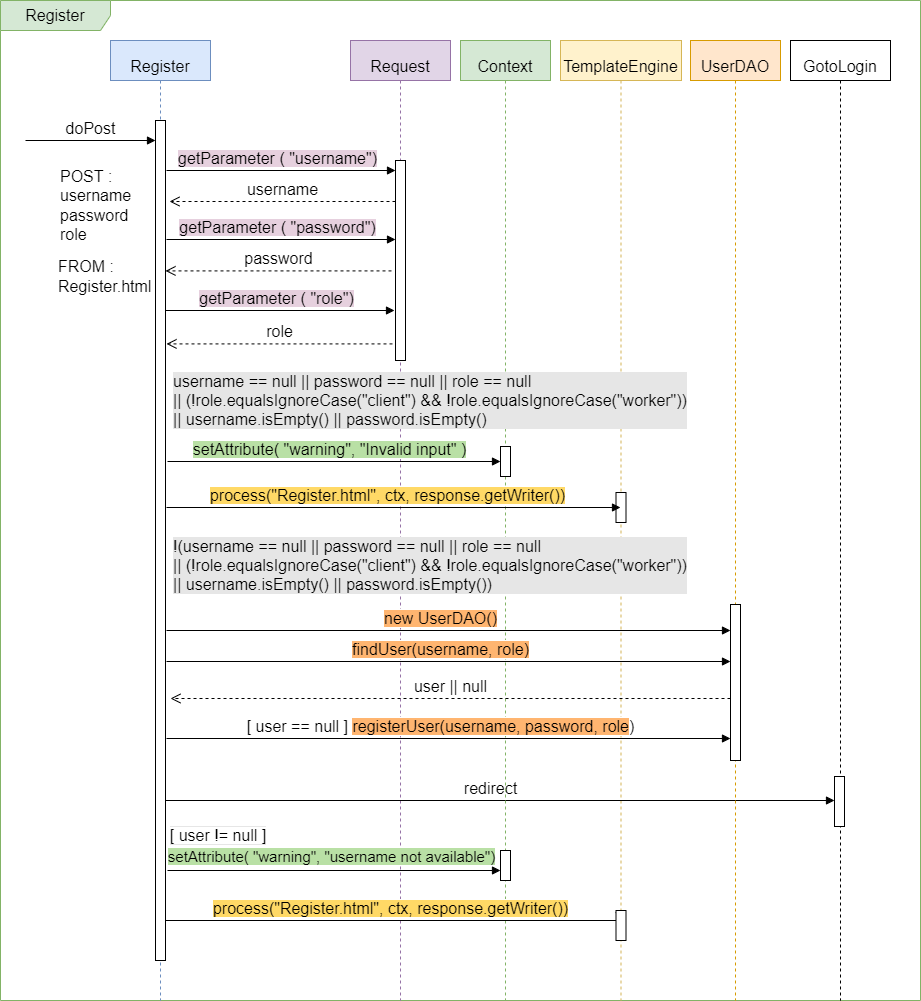
\includegraphics[width=1\textwidth]{PureHTML_images/Register.png}
	\caption{Event - Register}
	\label{figure:register_sd}
\end{figure}
\noindent \textbf{Controlli:}\\
\noindent \textbf{Server:} 
\noindent Viene controllato che :
\begin{enumerate}
\item I parametri della form non siano nulli o vuoti ( username - password - ruolo ).
\item Che all'interno del DB non esista un altro utente con lo stesso ruolo, avente lo stesso username.
\end{enumerate}



\subsubsection{GotoClientHome}
\begin{figure}[h!]
	\centering
	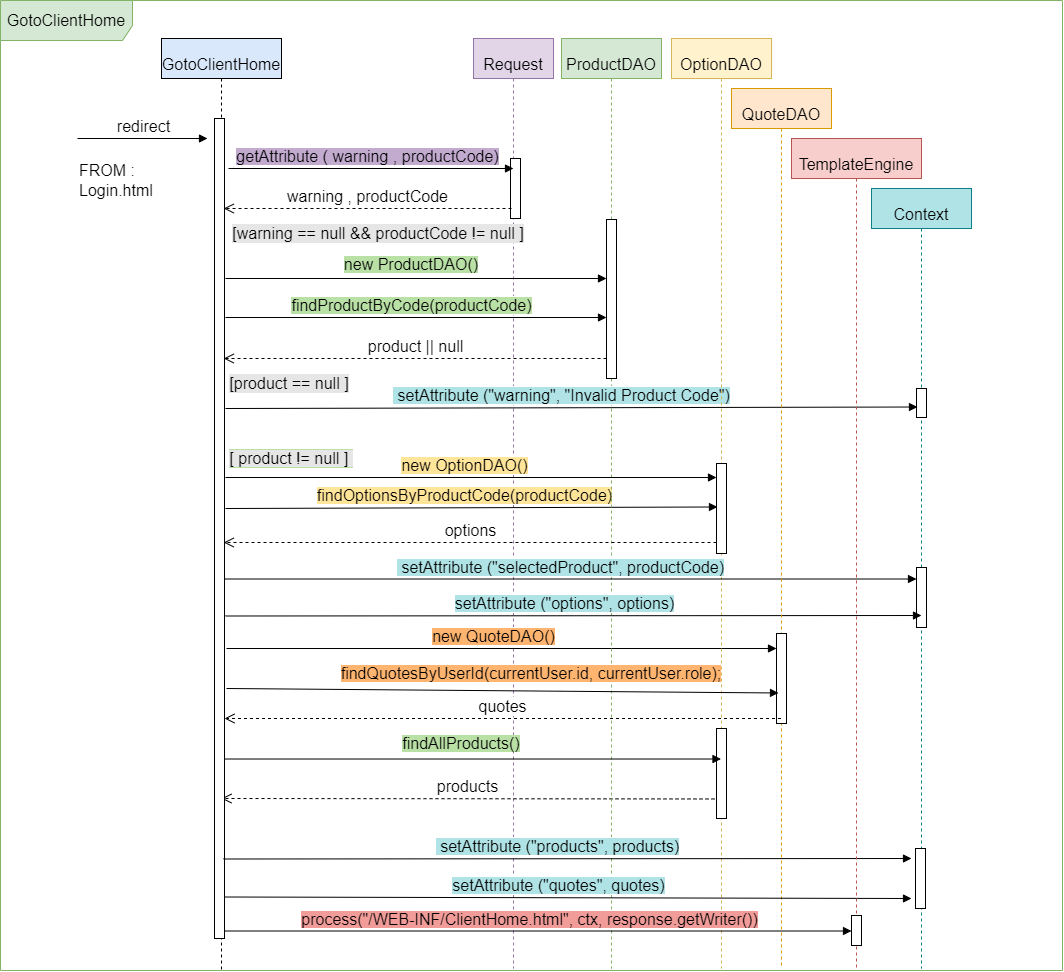
\includegraphics[width=1\textwidth]{PureHTML_images/GotoClientHome.png}
	\caption{Event - Go to Client Home}
	\label{figure:gotoclienthome_sd}
\end{figure}
\noindent \textbf{Controlli:}\\
\noindent \textbf{Server:} 
\noindent Al ricaricamento della pagina, dopo la selezione del prodotto per la richiesta di un nuovo preventivo, viene controllato che :
\begin{enumerate}
\item L'id del prodotto, se selezionato, sia in un formato numerico e corrisponda ad un id effetivamente presente nel DB.
\end{enumerate}
\newpage
\subsubsection{GotoWorkerHome}
\begin{figure}[h!]
	\centering
	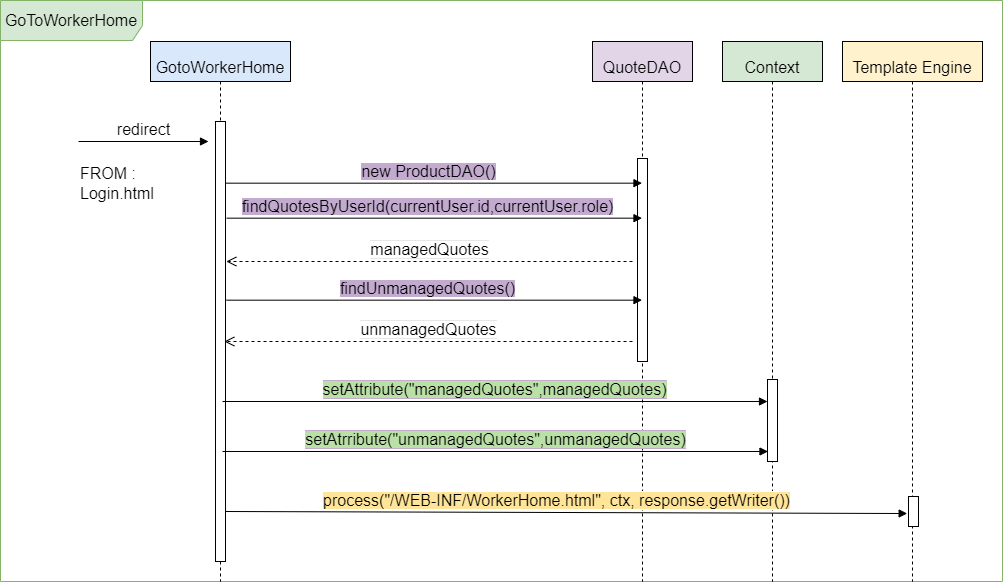
\includegraphics[width=1\textwidth]{PureHTML_images/GotoWorkerHome.png}
	\caption{Event - Go to Worker Home}
	\label{figure:gotoworkerhome_sd}
\end{figure}
\noindent \textbf{Controlli:}\\
\noindent \textbf{Server:} 
\noindent Dato che la raccolta dei dati necessari per la visualizzazione della pagina non dipendono da nessun parametro di input, ma solo dall'id dello user presente nella sessione, non vengono effettuati controlli aggiuntivi a quelli 
già fatti dai filtri ovvero: che un utente sia effettivamente loggato e che quest'ultimo sia effetivamente un worker.
\newpage
\subsubsection{GotoQuoteDetails}
\begin{figure}[h!]
	\centering
	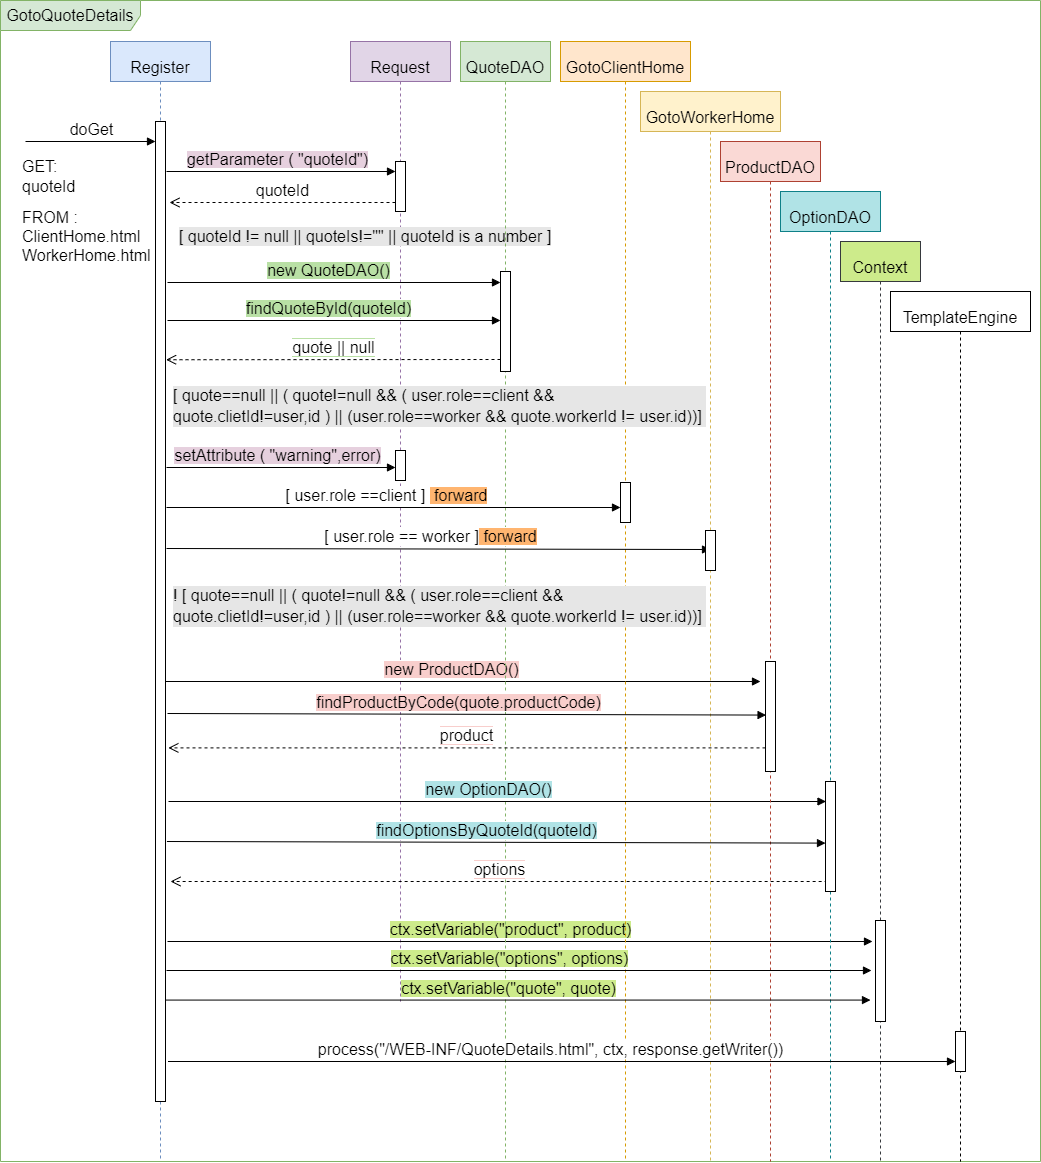
\includegraphics[width=1\textwidth]{PureHTML_images/GotoQuoteDetails.png}
	\caption{Event - Go to Quote Details}
	\label{figure:gotoquotedetails_sd}
\end{figure}
\noindent \textbf{Controlli:}\\
\noindent \textbf{Server:} 
\noindent Viene controllato che :
\begin{enumerate}
\item L'id del prodotto non sia nullo, vuoto, sia in un formato numerico e che corrisponda ad un id effetivamente presente nel DB.
\item Che lo user presente nella sessione abbia l'autorizzazione per visualizzare i dettagli del preventivo.
\end{enumerate}
\newpage
\subsubsection{CreateQuote}
\begin{figure}[h!]
	\centering
	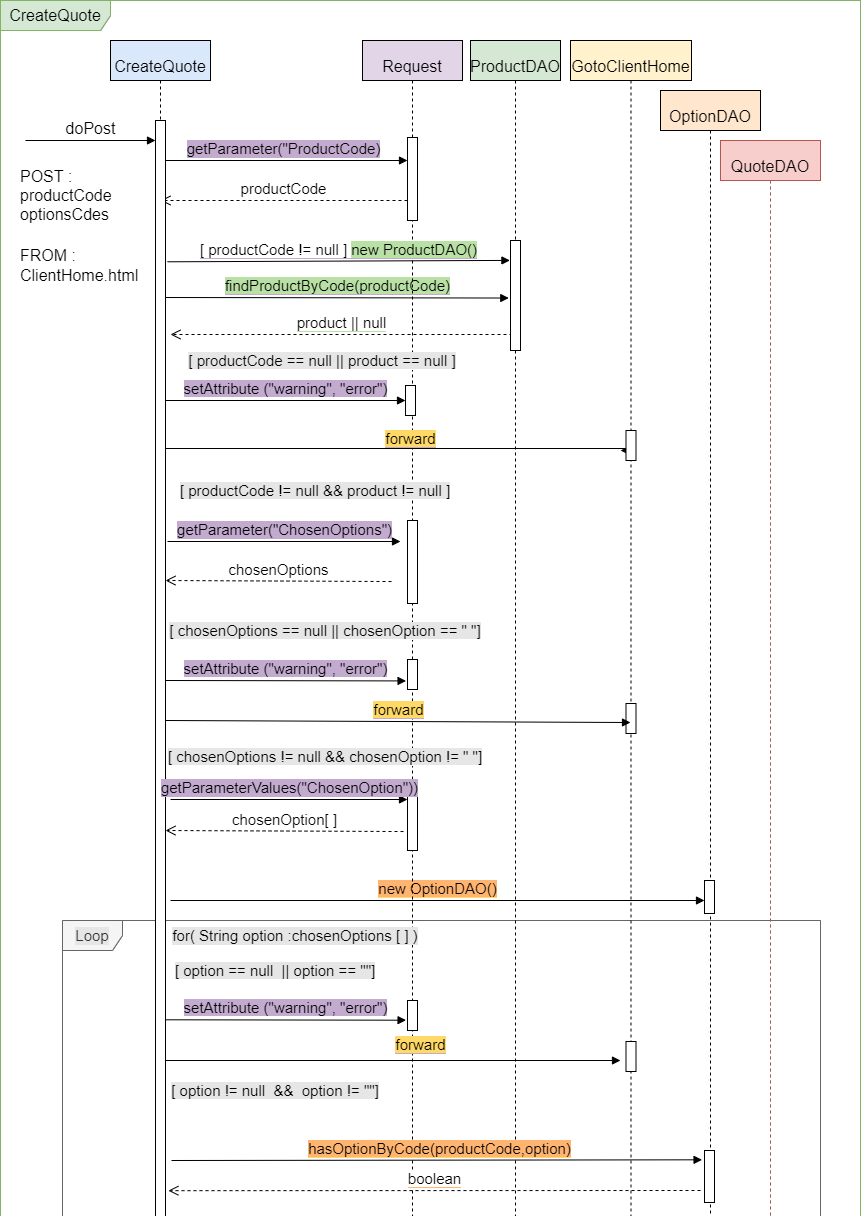
\includegraphics[width=1\textwidth]{PureHTML_images/CreateQuote1.png}
	\label{figure:createquote1_sd}
\end{figure}
\newpage
\begin{figure}[h!]
	\centering
	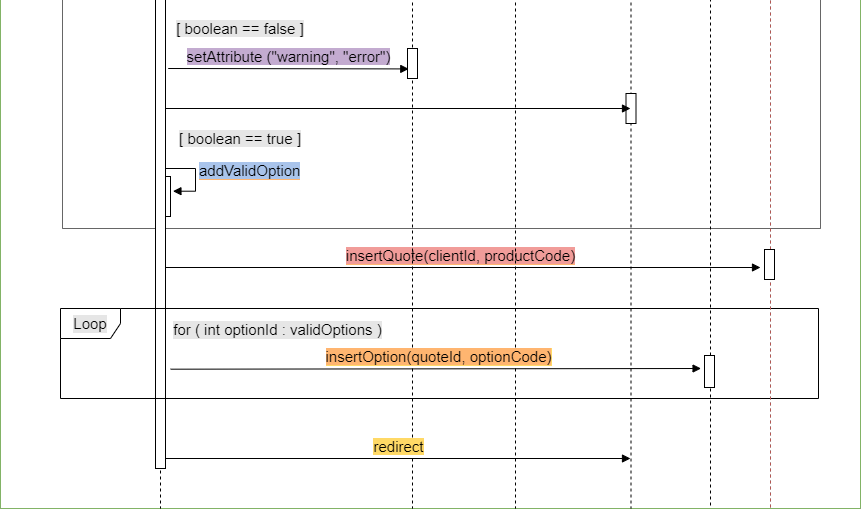
\includegraphics[width=1\textwidth]{PureHTML_images/CreateQuote2.png}
	\caption{Event - Create Quote}
	\label{figure:createquote2_sd}
\end{figure}
\noindent \textbf{Controlli:}

\noindent \textbf{HTML:} \\ La scelta di almeno un'opzione per la creazione del preventivo è obbligatoria.

\noindent \textbf{Server:} 

\noindent Viene controllato che :
\begin{enumerate}
\item L'id del prodotto non sia nullo, vuoto, sia in un formato numerico e che corrisponda ad un id effetivamente presente nel DB.
\item Il parametro \verb|chosenOption| non sia nullo o vuoto. Inoltre viene controllato che ogni elemento dell'array non sia nullo, vuoto , sia in formato numerico e corrisponda effetivamente ad una opzione
disponibile per il prodotto selezionato.
\end{enumerate}
\newpage
\subsubsection{UpdatePrice}
\begin{figure}[h!]
	\centering
	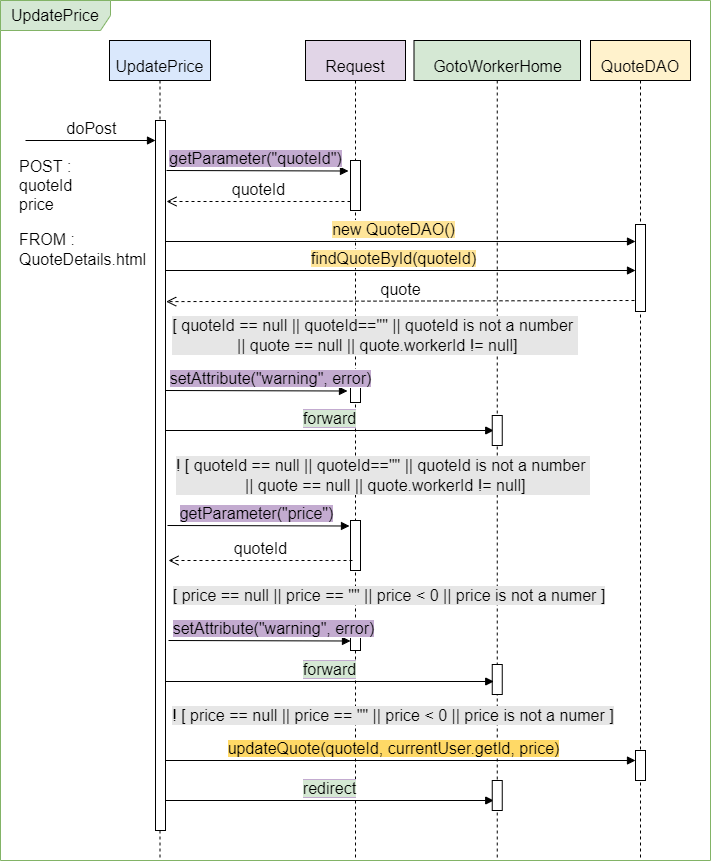
\includegraphics[width=1\textwidth]{PureHTML_images/UpdatePrice.png}
	\caption{Event - Update Price}
	\label{figure:updateprice_sd}
\end{figure}
\noindent \textbf{Controlli:}\\
\noindent \textbf{Server:} 
\noindent Viene controllato che :
\begin{enumerate}
\item L'id del prodotto non sia nullo, vuoto, sia in un formato numerico e che corrisponda ad un id effetivamente presente nel DB.
\item Che il preventivo non sia già stato prezzato da un altro worker.
\item Che il prezzo inserito non sia nullo,vuoto, sia in un formato numerico e maggiore di 0.
\end{enumerate}

\newpage
\section{Gestione Preventivi - RIA}
\subsection{Analisi dei dati per il database}
Si realizzi un’applicazione client server web che modifica le specifiche precedenti (subsection \ref{sub: Analisi dei dati per il database}) come segue:
\begin{itemize}
\item La registrazione controlla la validità sintattica dell’indirizzo di \textbf{\textcolor{myGreen}{email}} e l’uguaglianza tra i campi “password” e “ripeti password”, anche a lato client.
\item Dopo il login, l’intera applicazione è realizzata con un’unica pagina per ciascuno dei ruoli: una pagina singola per il ruolo di cliente e una pagina singola per il ruolo di impiegato.
\item Ogni interazione dell’utente è gestita senza ricaricare completamente la pagina, ma produce l’invocazione asincrona del server e l’eventuale modifica del contenuto da aggiornare a seguito dell’evento.
\item Nella pagina del cliente, la scelta del prodotto comporta la successiva visualizzazione delle opzioni senza produrre un’ulteriore chiamata al server.
\item L’invio del preventivo da parte del cliente deve produrre la verifica dei dati anche a lato client (almeno un’opzione scelta).
\item Nella pagina dell’impiegato, il controllo del prezzo (non nullo e maggiore di zero) deve essere fatto anche a lato client.
\item Eventuali errori a lato server devono essere segnalati mediante un messaggio di allerta all’interno della pagina del cliente o dell’impiegato.\\
\end{itemize}
\noindent \textbf{\textcolor{red}{Entities}, \textcolor{myGreen}{attributes}, \textcolor{myBlue}{relationships}}
\subsection{Database Design}
\subsection{Local Database schema}
\subsection{Analisi dei dati per i requisiti dell'applicazione}
Si realizzi un’applicazione client server web che modifica le specifiche precedenti (subsection \ref{sub: Analisi dei dati per i requisiti dell'applicazione}) come segue:
\begin{itemize}
\item La registrazione controlla la validità sintattica dell’indirizzo di email e l’uguaglianza tra \textbf{\textcolor{myGreen}{i campi “password” e “ripeti password”}}, anche a lato client.
\item Dopo il \textbf{\textcolor{red}{login}}, l’intera applicazione è realizzata con un’unica pagina per ciascuno dei ruoli: \textbf{\textcolor{red}{una pagina singola per il ruolo di cliente}} e \textbf{\textcolor{red}{una pagina singola per il ruolo di impiegato}}.
\item Ogni interazione dell’utente è gestita senza ricaricare completamente la pagina, ma produce l’invocazione asincrona del server e l’eventuale modifica del contenuto da aggiornare a seguito dell’evento.
\item Nella pagina del cliente, \textbf{\textcolor{myBlue}{la scelta del prodotto}} comporta la successiva \textbf{\textcolor{myBrown}{visualizzazione delle opzioni}} senza produrre un’ulteriore chiamata al server.
\item \textbf{\textcolor{myBlue}{L’invio del preventivo}} da parte del cliente deve produrre la \textbf{\textcolor{myBrown}{verifica dei dati}} anche a lato client (almeno un’opzione scelta).
\item Nella pagina dell’impiegato, il controllo del prezzo (non nullo e maggiore di zero) deve essere fatto anche a lato client.
\item Eventuali errori a lato server devono essere segnalati mediante un messaggio di allerta all’interno della pagina del cliente o dell’impiegato.\\
\end{itemize}
\noindent \textbf{\textcolor{red}{Pages(views)}, \textcolor{myGreen}{views components}, \textcolor{myBlue}{events}, \textcolor{myBrown}{actions}}
\subsection{Completamento delle specifiche}
\subsection{Sommario}
\subsubsection{Viste e componenti}
\begin{itemize}
	\item \textbf{Login Page}
	\begin{itemize}
		\item \textbf{Login Form}
		\begin{itemize}
			\item Email Input
			\item Password Input
			\item Login Button
			\item Register Now Anchor
		\end{itemize}
		\item \textbf{Register Form}
		\begin{itemize}
			\item Username Input
			\item Email Input
			\item Password Input
			\item Repeat Password Input
			\item Login Button
			\item Go to Login Anchor
		\end{itemize}
	\end{itemize}
	\item \textbf{Client Page}
	\begin{itemize}
		\item \textbf{CreateQuoteForm}
		\begin{itemize}
			\item Products List
			\item Options List
			\item Request Quote Button
		\end{itemize}
		\item \textbf{QuotesList}
		\begin{itemize}
			\item Quote Details
		\end{itemize}
		\item \textbf{Logout Button}
	\end{itemize}
	\item \textbf{Worker Page}
	\begin{itemize}
	\item \textbf{Managed Quotes List}
	\begin{itemize}
		\item Quote Details
	\end{itemize}
	\item \textbf{Unmanaged Quotes List}
	\begin{itemize}
		\item Quote Details
		\item Price Input
		\item Update Price Button
	\end{itemize}
		\item \textbf{Logout Button}
	\end{itemize}
\end{itemize}
\subsubsection{Eventi e azioni}
\begin{itemize}
	\item \textbf{Login Page}
	\begin{itemize}
		\item Click LoginButton -> verifica delle credenziali - apertura Client/WorkerPage
		\item RegisterNow -> visualizzazione form con i campi per la registrazione
		\item Click RegiaterButton -> verifica validità degli input - creazione account dello User - ritorno alla form di login
		\item Click GotoLogin -> ritorno alla form di login
	\end{itemize}
	\item \textbf{Client Page}
	\begin{itemize}
		\item Click su un prodotto -> visualizzazione senza ricaricamento della pagine delle opzioni relative al prodotto scelto
		\item Click sul bottone RequestQuote -> verifica validità degli input / aggiunta del prevetivo alla lista 
		\item Click sul preventivo -> visualizzazione/chiusura dettagli del preventivo
		\item Click LogoutButton -> logout
	\end{itemize}
	\item \textbf{Worker Page}
	\begin{itemize}
		\item Click preventivo non gestito -> visualizzazione dettagli preventivo - visualizzazione input per inserimento prezzo / chiusura dettagli input 
		\item Click UpdatePriceButton -> verifica validità input - aggiornamento prezzo del preventivo 
		\item Click preventivo gestito -> visualizzazione / chiusura dettagli del preventivo selezionato 
		\item Logout -> logout 
	\end{itemize}
\end{itemize}
\newpage
\subsection{Application Desing}
\begin{figure}[h!]
	\centering
	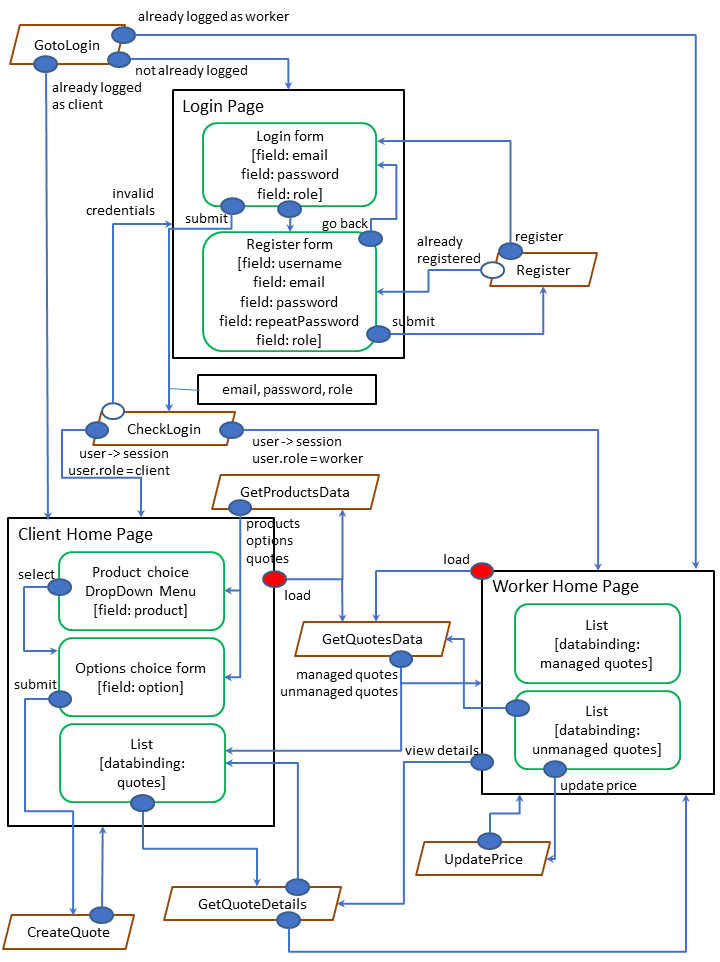
\includegraphics[width=1\textwidth]{RIA_images/ifmlRIA.png}
	\caption{Event - IFML Diagram}
	\label{figure:ifmlRIA}
\end{figure}
\subsection{Eventi e azioni}
\begin{table}[h!]  
	\centering
	\begin{tabu} to 1.0\textwidth {|X[c]|X[c]|X[c]|X[c]|}
		\hline
		\multicolumn{2}{|c|}{\textbf{Client Side}} & \multicolumn{2}{c|}{\textbf{Server Side}} \\
		\hline
		\textbf{Evento} & \textbf{Azione} & \textbf{Evento} & \textbf{Azione} \\
		\hline
		login -> login form -> submit \vspace{2mm} & Controllo dati \vspace{2mm} & POST email, password e ruolo \vspace{2mm} &  Controllo credenziali \vspace{2mm}\\
		\hline
		login -> register form -> submit \vspace{2mm} & Controllo dati \vspace{2mm} & POST username, email, password e ruolo \vspace{2mm} & Controllo validità credenziali \vspace{2mm} \\
		\hline
		Client Page -> load \vspace{2mm} & Aggiorna view con elenco dei prodotti e lista dei preventivi del cliente \vspace{2mm} & GET \vspace{2mm} & Estrazione dei prodotti, delle rispettive opzioni e dei preventivi \vspace{2mm} \\
		\hline
		Client Page -> scelta prodotto \vspace{2mm} & Mostra le opzioni disponibili per il prodotto scelto \vspace{2mm} & & \\
		\hline
		Client Page -> richiedi preventivo \vspace{2mm} & Controllo validità dati \vspace{2mm} & POST  prodotto e opzioni \vspace{2mm} & Creazione preventivo e inserimento nel db \vspace{2mm}\\
		\hline
		Client Page -> elenco preventivi -> click \vspace{2mm} & Mostra dettagli del preventivo \vspace{2mm} & & \\
		\hline
		Worker Page -> load \vspace{2mm} & Aggiorna view con la lista dei preventivi gestiti dal worker e la lista dei preventivi non ancora gestiti \vspace{2mm} & GET \vspace{2mm} & Estrazione dei preventivi \vspace{2mm}\\
		\hline
		Worker Page -> update price \vspace{2mm} & Controlla la validità del prezzo \vspace{2mm} & POST preventivo e prezzo \vspace{2mm} & Aggiornamento del prezzo del preventivo \vspace{2mm}\\
		\hline
		Worker Page -> elenco preventivi -> click \vspace{2mm} & Mostra dettagli del preventivo \vspace{2mm} & & \\
		\hline
		Logout \vspace{2mm} & & GET \vspace{2mm} & Terminazione della sessione \vspace{2mm}\\
		\hline
	\end{tabu}
\end{table}
\subsection{Controller and Event Handler}
\begin{table}[h!]  
	\centering
	\begin{tabu} to 1.0\textwidth {|X[c]|X[c]|X[c]|X[c]|}
		\hline
		\multicolumn{2}{|c|}{\textbf{Client Side}} & \multicolumn{2}{c|}{\textbf{Server Side}} \\
		\hline
		\textbf{Evento} & \textbf{Controllore} & \textbf{Evento} & \textbf{Controllore} \\
		\hline
		login -> login form -> submit \vspace{2mm} & Function makeCall \vspace{2mm} & POST email, password e ruolo \vspace{2mm} &  CheckLogin \vspace{2mm}\\
		\hline
		login -> register form -> submit \vspace{2mm} & Function makeCall \vspace{2mm} & POST username, email, password e ruolo \vspace{2mm} & Register \vspace{2mm} \\
		\hline
		Client Page -> load \vspace{2mm} & Function PageHandler \vspace{2mm} & GET \vspace{2mm} & GetProductsData and GetQuotesData \vspace{2mm} \\
		\hline
		Client Page -> scelta prodotto \vspace{2mm} & Function OptionsList.show \vspace{2mm} & & \\
		\hline
		Client Page -> richiedi preventivo \vspace{2mm} & Function OptionsList.createQuote \vspace{2mm} & POST  prodotto e opzioni \vspace{2mm} & CreateQuote \vspace{2mm}\\
		\hline
		Client Page -> elenco preventivi -> click \vspace{2mm} & Function QuotesList.addDetails \vspace{2mm} & GET quote id & GetQuoteDetails\\
		\hline
		Worker Page -> load \vspace{2mm} & Function PageHandler \vspace{2mm} & GET \vspace{2mm} & GetQuotesData\vspace{2mm}\\
		\hline
		Worker Page -> update price \vspace{2mm} & Function QuotesList.updatePrice \vspace{2mm} & POST preventivo e prezzo \vspace{2mm} & UpdatePrice \vspace{2mm}\\
		\hline
		Worker Page -> elenco preventivi -> click \vspace{2mm} & Function QuotesList.addDetails \vspace{2mm} & GET quote id & GetQuoteDetails\\
		\hline
		Logout \vspace{2mm} & & GET \vspace{2mm} & Logout(servlet) \vspace{2mm}\\
		\hline
	\end{tabu}
\end{table}
\subsection{Server Side: DAO \& Model Object}
\begin{itemize}
	\item \textbf{Model Objects (Beans)}
	\begin{itemize}
		\item Option
		\item Product
		\item Quote
		\item User
	\end{itemize}
	\item \textbf{Data Access Objects (Classes)}
	\begin{itemize}
		\item \textbf{OptionDAO}
		\begin{itemize}
			\item boolean hasOptionByCode(int productCode, int optionCode);
			\item List<Option> findOptionsByProductCode(int productCode);
			\item List<Option> findOptionsByQuoteId(int quoteId);
			\item void insertOption(int quoteId, int optionCode);
		\end{itemize}
		\item \textbf{ProductDAO}
		\begin{itemize}
			\item List<Product> findAllProducts();
			\item Product findProductByCode(int code);
		\end{itemize}
		\item \textbf{QuoteDAO}
		\begin{itemize}
			\item List<Quote> findQuotesByUserId(int userId, String role);
			\item Quote findQuoteById(int quoteId);
			\item List<Quote> findUnmanagedQuotes();
			\item int insertQuote(int clientId, int productCode);
			\item void updateQuote(int quoteId, int workerId, int price);
		\end{itemize}
		\item \textbf{UserDAO}
		\begin{itemize}
			\item User findUser(String email, String password, String role);
			\item User findUserToRegister(String username, String email, String role);
			\item User findClientById(int clientId);
			\item void registerUser(String username, String password, String role);
		\end{itemize}
	\end{itemize}
	\item \textbf{Controllers (Servlets)}
	\begin{itemize}
		\item GotoLogin
		\item CheckLogin
		\item Register
		\item GetProductsData
		\item GetQuotesData
		\item CreateQuote
		\item GetQuoteDetails
		\item UpdatePrice
		\item Logout
	\end{itemize}
	\item \textbf{Filters}
	\begin{itemize}
		\item SessionChecker
		\item ClientChecker
		\item WorkerChecker
	\end{itemize}
	\item \textbf{Views (Templates)}
	\begin{itemize}
		\item Login.html
		\item ClientHome.html
		\item WorkerHome.html
	\end{itemize}
\end{itemize}
\subsection{Client Side: view \& view components}
\begin{itemize}
	\item \textbf{LoginManagement.js}
	\begin{itemize}
	\item returnToLogin(): modifica gli elementi della form per passare dalla Register form alla Login form;
	\item checkEmail(email): verifica validità email;
	\item loginButton.addEventListener
	\item openRegister.addEventListener
	\end{itemize}
	\item \textbf{PageHandler.js}
	\begin{itemize}
		\item \textbf{OptionsList}
		\begin{itemize}
		\item reset(): rende invisibile le opzioni;
		\item clear(): toglie dalla select tutte le options;
		\item show(): visualizza le opzioni relative al prodotto selezionato;
		\item createQuote(): verifica la validità degli input della form - registra il preventivo;
		\item checkChosenOptions (): verifica validità opzioni scelte;
		\end{itemize}
		\item \textbf{CreateQuoteForm}
		\begin{itemize}
		\item getDropDownButton(): restituisce il bottone che gestisce la scelta dei prodotti;
		\item show(): richiede al server i prodotti disponibili;
		\item update(): aggiorna la lista dei prodotti da visualizzare;
		\end{itemize}
		\item \textbf{QuoteList}
		\begin{itemize}
			\item show(): richiede al server la lista dei preventivi richiesti dal client/gestiti dal Worker/non gestiti;
			\item update(): aggiorna la lista dei preventivi;
			\item addDetails(): richiede al server i dettagli del preventivo selezionato;
			\item updateDetails(): visualizza i dettagli del preventivo;
			\item updatePrice(): verifica la validità dell'input - aggiorna il prezzo del preventivo;
			\item checkCorrectPrice(): verifica l'input - mostra un warning in caso di errore;
			\item clear(): rimuove tutti i preventivi dalla lista;
		\end{itemize}
		\item \textbf{PageHandler}
		\begin{itemize}
			\item start(): crea e inizializza i componenti dell'interfaccia;
		\end{itemize}
	\end{itemize}
\end{itemize}
\subsection{Events}
\subsubsection{Login}
\begin{figure}[h!]
	\centering
	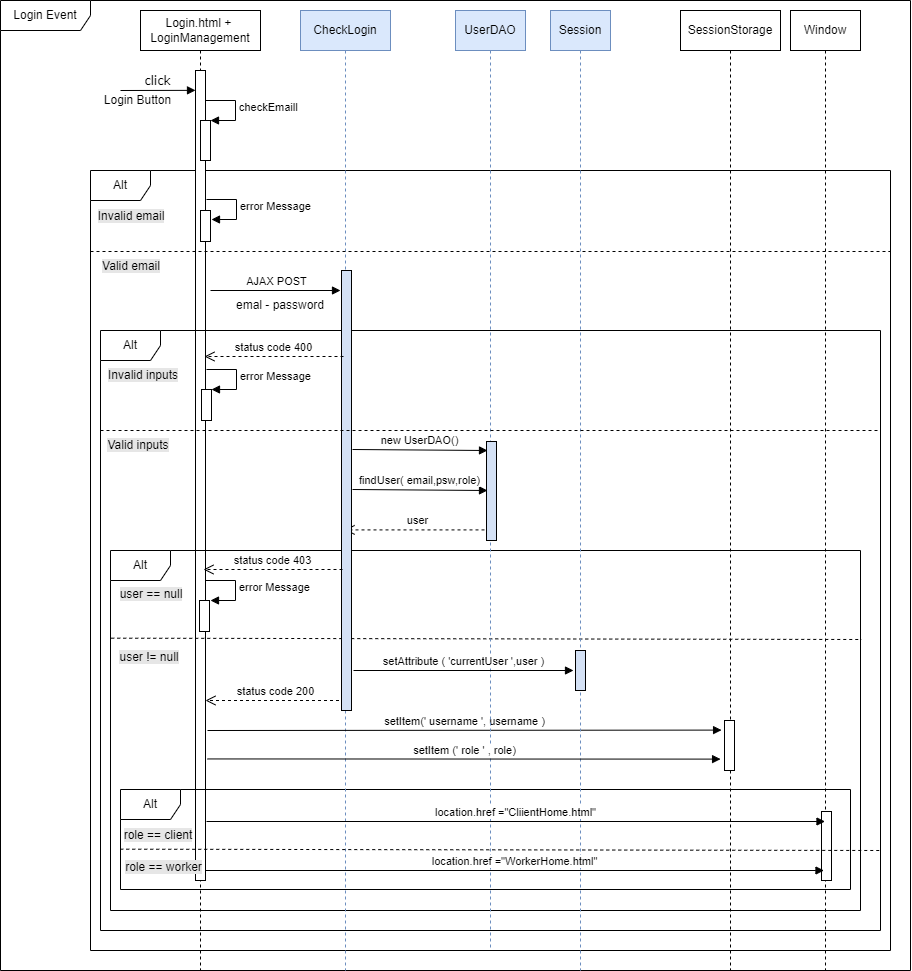
\includegraphics[width=1\textwidth]{RIA_images/LoginEvent.png}
	\caption{Event - Login}
	\label{figure:LoginRIA}
\end{figure}
\subsubsection{Register}
\begin{figure}[h!]
	\centering
	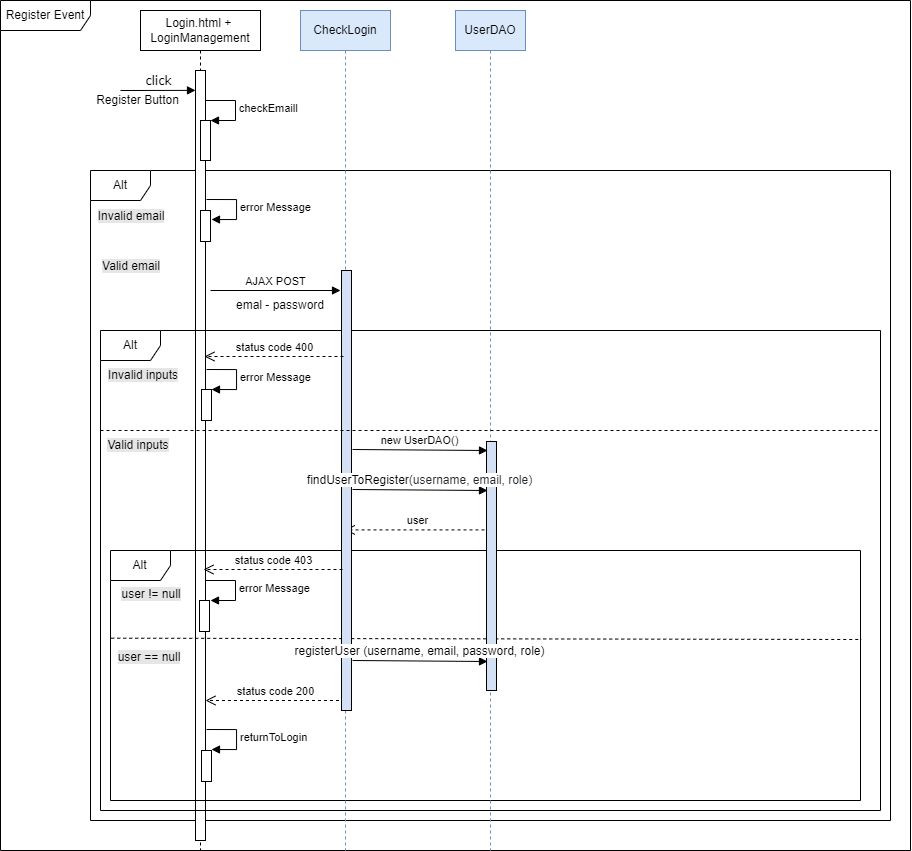
\includegraphics[width=1\textwidth]{RIA_images/RegisterEvent.png}
	\caption{Event - Register}
	\label{figure:RegisterRIA}
\end{figure}
\subsubsection{View Options}
\begin{figure}[h!]
	\centering
	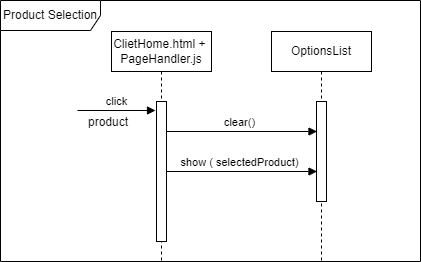
\includegraphics[width=0.5\textwidth]{RIA_images/ViewOptionsEvent.png}
	\caption{Event - View Options}
	\label{figure:ViewOptionsRIA}
\end{figure}
\subsubsection{Create Quote}
\begin{figure}[h!]
	\centering
	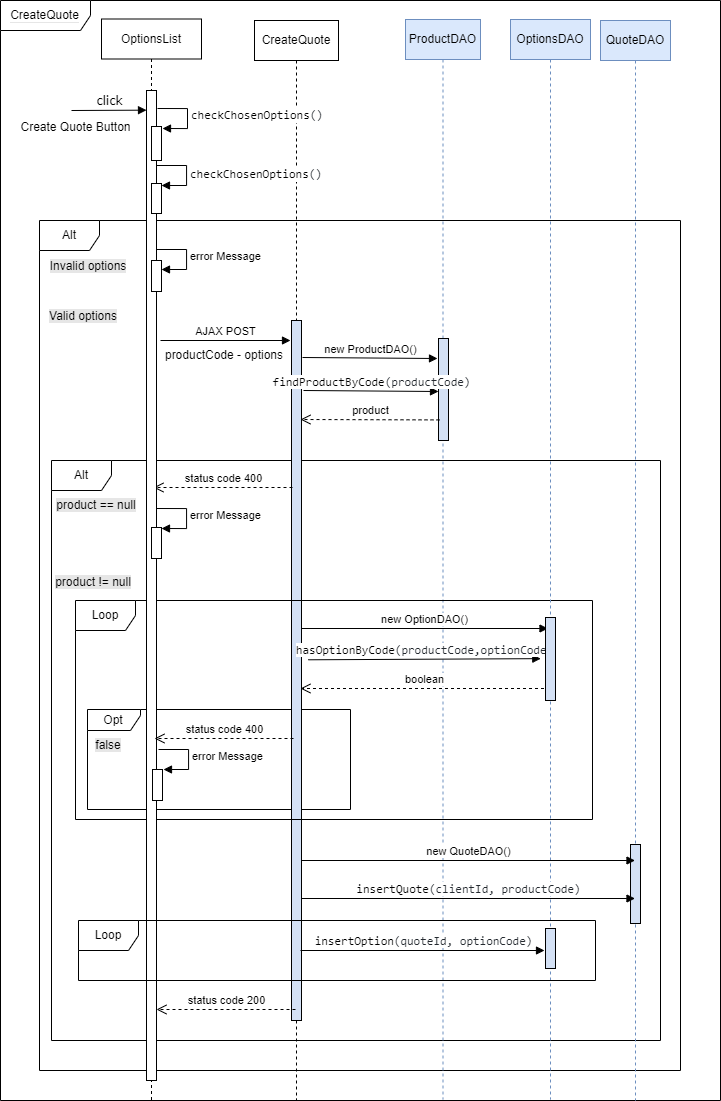
\includegraphics[width=1\textwidth]{RIA_images/CreateQuote.png}
	\caption{Event - Create Quote}
	\label{figure:CreateQuoteRIA}
\end{figure}
\subsubsection{Update Price}
\begin{figure}[h!]
	\centering
	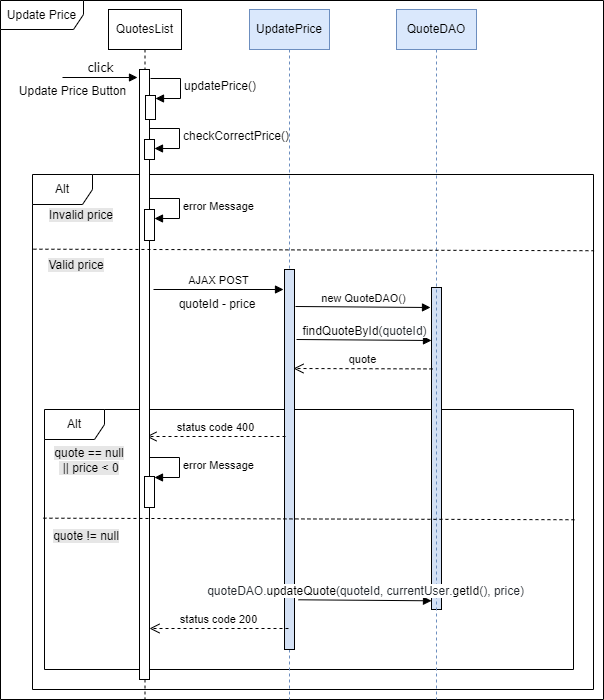
\includegraphics[width=1\textwidth]{RIA_images/UpdatePrice.png}
	\caption{Event - Update Price}
	\label{figure:UpdatePriceRIA}
\end{figure}
\end{document}